\documentclass[11pt]{article}

\usepackage{geometry}
\geometry{
    top = 1 in,
    bottom = 1in,
    right = 1in,
    left = 1in,
}

\usepackage{amsmath}
\usepackage{graphicx}
\usepackage{parskip}

\title{Assembly Project: Report 2}

\author{Wangzheng Jiang 1008109574; Yahya Elgabra 1008553030}

\begin{document}
\maketitle

\section{Constants and Variables in Memory}

Note: All data stored below are of data type ``word''.
\begin{enumerate}

\item Address of the display: \verb+ADDR_DSPL = 0x10008000+
\item Address of keyboard input: \verb+ADDR_KBRD = 0xffff0000+
\\
\item Color of the side walls (and the top bar): \verb+COLOR_WALLS = 0x00888888+
\item Thickness (in units) of the top bar: \verb+TOP_BAR_THICKNESS = 8+
\item Thickness (in units) of the side walls: \verb+SIDE_WALL_THICKNESS = 2+
\item Gap (in units) between the top bar and the first row of bricks: \verb+TOP_GAP_THICKNESS = 8+
\\
\item Thickness (in units) of a row of bricks: \verb+BRICK_ROW_THICKNESS = 2+
\item The number of rows of bricks: \verb+BRICK_ROW_AMOUNT = 7+
\item An array containing the colors of each row of bricks: \\ \verb+BRICK_COLORS = [0x008062e0, 0x007173c6, 0x006283ac, 0x00539492,+\\ \verb+                0x0043a577, 0x0034b55d, 0x0025c643]+
\\
\item The y-coordinate of the paddle (constant): \verb+PADDLE_Y = 61+
\item The x-coordinates of the paddle, these are variable, one stores the x-coordinate of the leftmost pixel of the paddle, one stores the rightmost. This enables us to adjust the length of the paddle, and makes it easier for us to update its position:\\ \verb+PADDLE_X_LEFT = 26+ ; \verb+PADDLE_X_RIGHT = 36+
\\
\item The y-coordinate of the paddle (constant): \verb+PADDLE_2_Y = 58+
\item The x-coordinates of the second paddle, these are variable, one stores the x-coordinate of the leftmost pixel of the paddle, one stores the rightmost. This enables us to adjust the length of the paddle, and makes it easier for us to update its position:\\ \verb+PADDLE_2_X_LEFT = 26+ ; \verb+PADDLE_2_X_RIGHT = 36+
\\
\item The position of the ball (this is a variable): \verb+BALL_X = 31+ ; \verb+BALL_Y = 56+
\item The movement vectors for the ball (each cycle the balls position are calculated as such: \verb%BALL_X = BALL_X + VEC_X% ; \verb%BALL_Y = BALL_Y + VEC_Y% ). For ease of calculation, \verb+VEC_X+ and \verb+VEC_Y+ can only be either 1 or -1:\\ \verb+VEC_X = 1+ ; \verb+VEC_Y = 1+
\\
\item The width of a single brick (constant): \verb+BRICK_WIDTH = 6+
\\
\item The players' score, each time a brick is hit the score increments by 1 (variable): \verb+SCORE = 0+
\\
\item The players' lives, each time the players lose, one of the hearts turn black:\\ \verb+LIVES = [0x00FF0000, 0x00FF0000, 0x00FF0000]+
	
\end{enumerate}

Data in Memory:

\begin{center}
	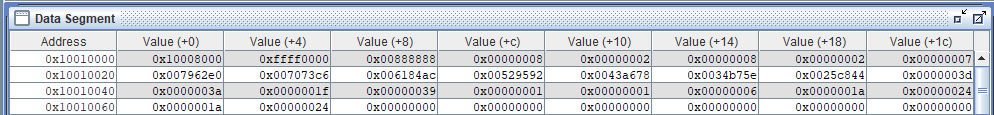
\includegraphics[scale=0.5]{project_report_2_data_hex}
	
	Data in Hexadecimal
	
	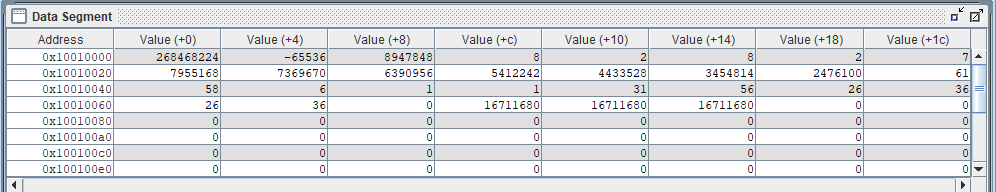
\includegraphics[scale=0.5]{project_report_2_data_dec}
	
	Data in Decimal
\end{center}

\section{Scene}

\begin{center}
	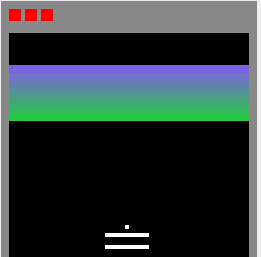
\includegraphics[scale=0.9]{project_report_2_scene}
\end{center}

\section{Collision Algorithm}

In each game cycle, we check the 4 pixels directly adjacent to the pixel where the ball is at: \verb%(BALL_X + 1, BALL_Y)%, \verb%(BALL_X - 1, BALL_Y)%, \verb%(BALL_X, BALL_Y + 1)%, \verb%(BALL_X, BALL_Y - 1)%. If any of the 4 pixels are not the default black background (0x00000000), then we have ``touched" something. 

And since we are only moving diagonally, the process is as follows:

If the ball is touching something on it's left or right, i.e. \verb%(BALL_X + 1, BALL_Y)% or \verb%(BALL_X - 1, BALL_Y)%, then we invert the sign of \verb+VEC_X+. (\verb+VEC_X = - VEC_X+) So that when we update the position of the ball using \verb%BALL_X += VEC_X%. It will go the opposite direction than where it was going.

Likewise, if the ball is touching something on it's top or bottom, i.e. \verb%(BALL_X, BALL_Y + 1)% or \verb%(BALL_X, BALL_Y - 1)%, then we invert the sign of \verb+VEC_Y+. (\verb+VEC_Y = - VEC_Y+) So that when we update the position of the ball using \verb%BALL_Y += VEC_Y%. It will go the opposite direction than where it was going.

These 2 cases can have either one applied, or both applied to the directional vectors of the ball.

\section{How to Play}

Buttons to play: 

Player 1: `a' for moving your pad to the left, `d' for moving your pad to the right

Player 2: `,' for moving your pad to the left, `.' for moving your pad to the right

`p' to pause, `p' to unpause and launch

'r' to reset

`q' to quit

Hit bricks with the ball to destroy them, each row of bricks requires 1 extra hit to be destroyed,press `p' to launch the ball, you can move your paddles and the ball before launching! Make sure not to let the ball reach the bottom of the screen or else you will lose a life! You win once you destroy all the bricks.

\section{Specifications}

This version of the project uses eMARS 4.7 as it makes the game run smoother and makes things easier to set up

\end{document}
